\chapter{Introduction} 
Organic semiconductors have a niche to fill across the landscape of electronic
device manufacturing due to the flexibility, processability, and cost of manufacturing. They have all ready
achieved commercial viability in organic light emitting
diodes (OLEDs) \cite{Song2020} and breakthroughs in organic field-effect transistors (OFETs)
indicate that that they are soon to folow \cite{Chen2020}. Exciting research is being done to provide stretchability, self-healing, and biodegradability for 
next generation medical devices \cite{Brutting2006}.
More generally, the solution processability of these materials allows for
cheaper manufacturing, the consumption of less rare elements, 
and the ability to assemble on curved substrates make the for a dizzying array of design possibilities. 
A survey of these materials, and 
other emerging organic electronic technologies, can be found the survey text 
Organic Electronic: Emerging Concepts and Technologies
\cite{FabioCicoiraEditor2013}. 

The methods used in this thesis are centrally motivated by, and justified for, 
the application of our workflow to materials
used in the design of organic photovoltaics (OPVs) for use in organic solar cells (OSCs). However, the methods are
not exclusively applicable to these materials and could be applied similarly to  supplement the engineering of any organic
electronic devices, like those mentioned above. 

OSCs can assist us in harnessing the power of the sun in ways not available to traditional cells. 
For example, researchers have exploited a unique feature of the physics the excitonic photoabsorbtion in 
organic materials.  Namely, that absorbtion spectrum
in these materials is relatively narrow ($\approx$300nm)
With this, they are able to tune the active layer material to absorb radiation right above or right below the
visible spectrum (into the NIR or UV spectrum respectively). This 
could allow for the production of windows that passively draw current while allowing in natural light. Semi-transparent OSCs have already
reached 11 \% efficeincy \cite{Brabec2020}. 

In our present work, we present results from an investigation of two OPV materials
used in the design of the active layer of organic solar cells (OSCs). P3HT, a
donor molecule, and ITIC, an acceptor molecule. With respect to organic electronic devices, `acceptors' are the
organic analogue of p-type inorganic semiconductors and `donors' the analogue
of the n-type.\ej{maybe a good place to talk about where they've been used before and how they're different.} We make this note because in the methods we describe a model of
a charge `hopping' from one molecule to another. And as we describe, our
investigation involves hops within a pure donor domain or within a pure
acceptor domain. A common point of confusion is distinguishing between which
molecules are donors or acceptors.
Any molecule can accept or donate a charge carrier OPV.
They merely receive their donor/acceptor designation as a result of how they
are primarily utilized in electronic devices. 

\begin{figure}[]
\centering
\begin{subfigure}{.5\textwidth}
    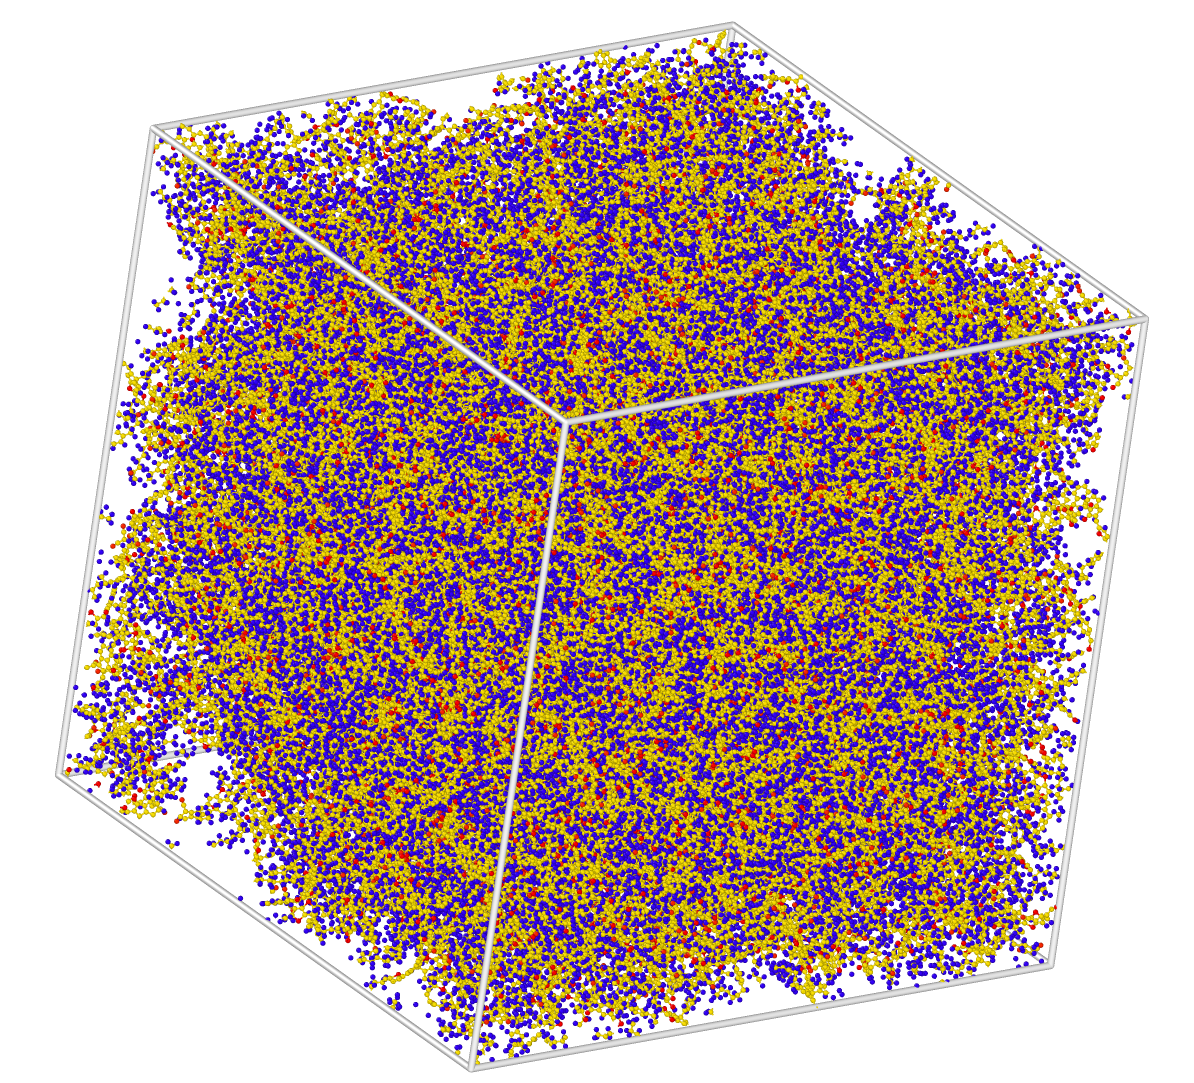
\includegraphics[width=\textwidth]{figures/ITIC.png}
\end{subfigure}%
\begin{subfigure}{.5\textwidth}
    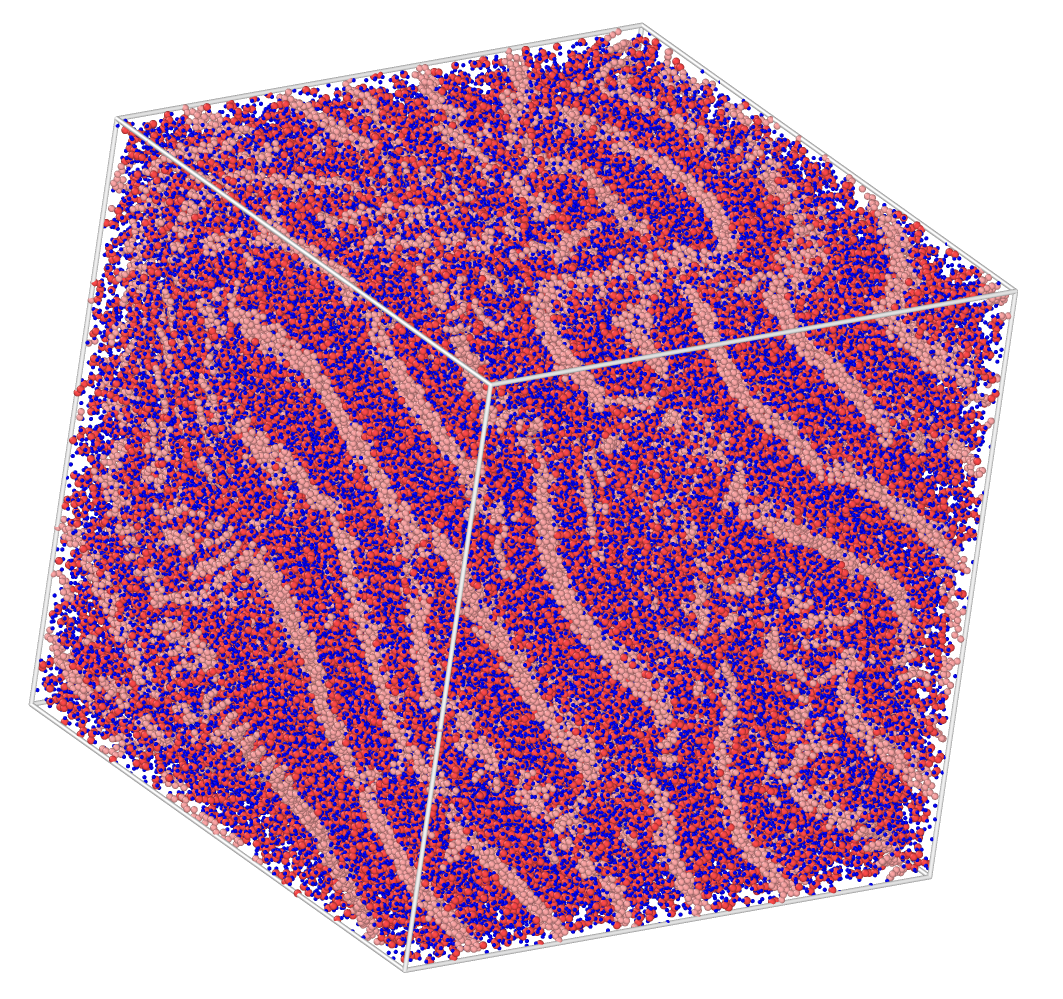
\includegraphics[width=\textwidth]{figures/P3HT.png}
\end{subfigure}
    \caption[short]{Left: 1000 molecule atomistic morhology of ITIC. Right: 1000 molecule atomistic simulation
    of P3HT}
\label{ITIC/P3HT}
\end{figure}


Two major breakthroughs have ushered us into the modern era of OSCs,
wherein effeciencies are approaching the milestone 20\% effeciency \cite{Liu2020b}.
These are the design of bulk heterojunction (BHJ) active layers and non-fullerene, fused-ring electron
acceptor (FREAs) molecules. 
\ej{expecting examples of how BHJ's were one breakthrough and how NFAs were another}

A fundemental physical difference in the nature of photoabsorbtion in inorganic and organic semiconduction materials necessitated the
invention of the BHJ. The coloumbic attraction, $V$, between the an excited
electron and the hole it leaves behind in the its molecular orbital
is given by Coulombs law as follows:

\begin{align}
    V  =  k_{e} \cdot \frac{e^{2}}{\epsilon_{r}}
\end{align}

where $k_{e}$ is Coulomb's constant and $e$ is charge of an electron. Relative permitivitty,
$\epsilon_{r}$, is a unitless quantity that describes a materials polarizability relative
to that of free space. That is, relative
permativity describes the readiness of a material
to polarize in response to an electric field. A
relative permitivitty of $~3$ in OPVs means that these materials are only $3$ times more polarizable than free space, which
is not all that polariazable. And, because the material occupying the space between electron and hole
is not willing (or able?) to fight back against the electric field created between them, they stick together and behave as a quasipartcle. 
This bound electron-hole quasiparticle is refered to herein as an exciton.

[Silicon has a relative permitivitty of ~12. not sure in need this i think its kinda understood]

This excitonic absorbtion introduces a unique design challenge.
That is, to extract a charge from the device, the exciton
must first be coerced apart. This coercion can take place at the interface between donor and acceptor molecules,
where the slight offset in energy levels creates a charge transfer state wherein it is more
energetically favorable for the donor to undergo electron transfer with an adjacent acceptor than
it is to radiatively decay to its ground state and photoemit.
However, after photoabsorbtion, the exciton must to diffuse to this interface for the charge to be
extracted. An exciton can diffuse roughly 10nm before relaxing \cite{clarke2010} \ej{Citation needed. There's some evidence from Bernie Yurke and others that excitons can travel further than 10nm in ordered morphologies, and so this 10nm number is an informed guess based on only opv materials (Maybe some articles by Darling or McGehee can unpack this?), and that perhaps our simulations can help us dispel if untrue.}
Producing a layer this small is untenable and further a thicker layer
is diserable to interact with as much of the ambeint radiation as possible so as to ``catch'' as many photons
as possbible. 

In 1986, Ching W. Tang
showed that, processed under the right conditions, a blend of donor and acceptor molecules can self-assemble
into what is termed Bulk Heterojunction (BHJ) microstructure \cite{Tang1986c}. 
The interlocking phases of donor accepter molecules, ensure
that an exciton will intersect with the boundary between accepter and donor domains, while also ensuring that
there
is a continuous escape route, albeit labyrinthine, for the free charges to travel on their way to their respective
electrodes. 

\ej{I didnt know if this meant real picture of bhj schematic but i made the latter
to refer to here as well as when i discuss the four stages of bhj}



\begin{figure}
    \center
    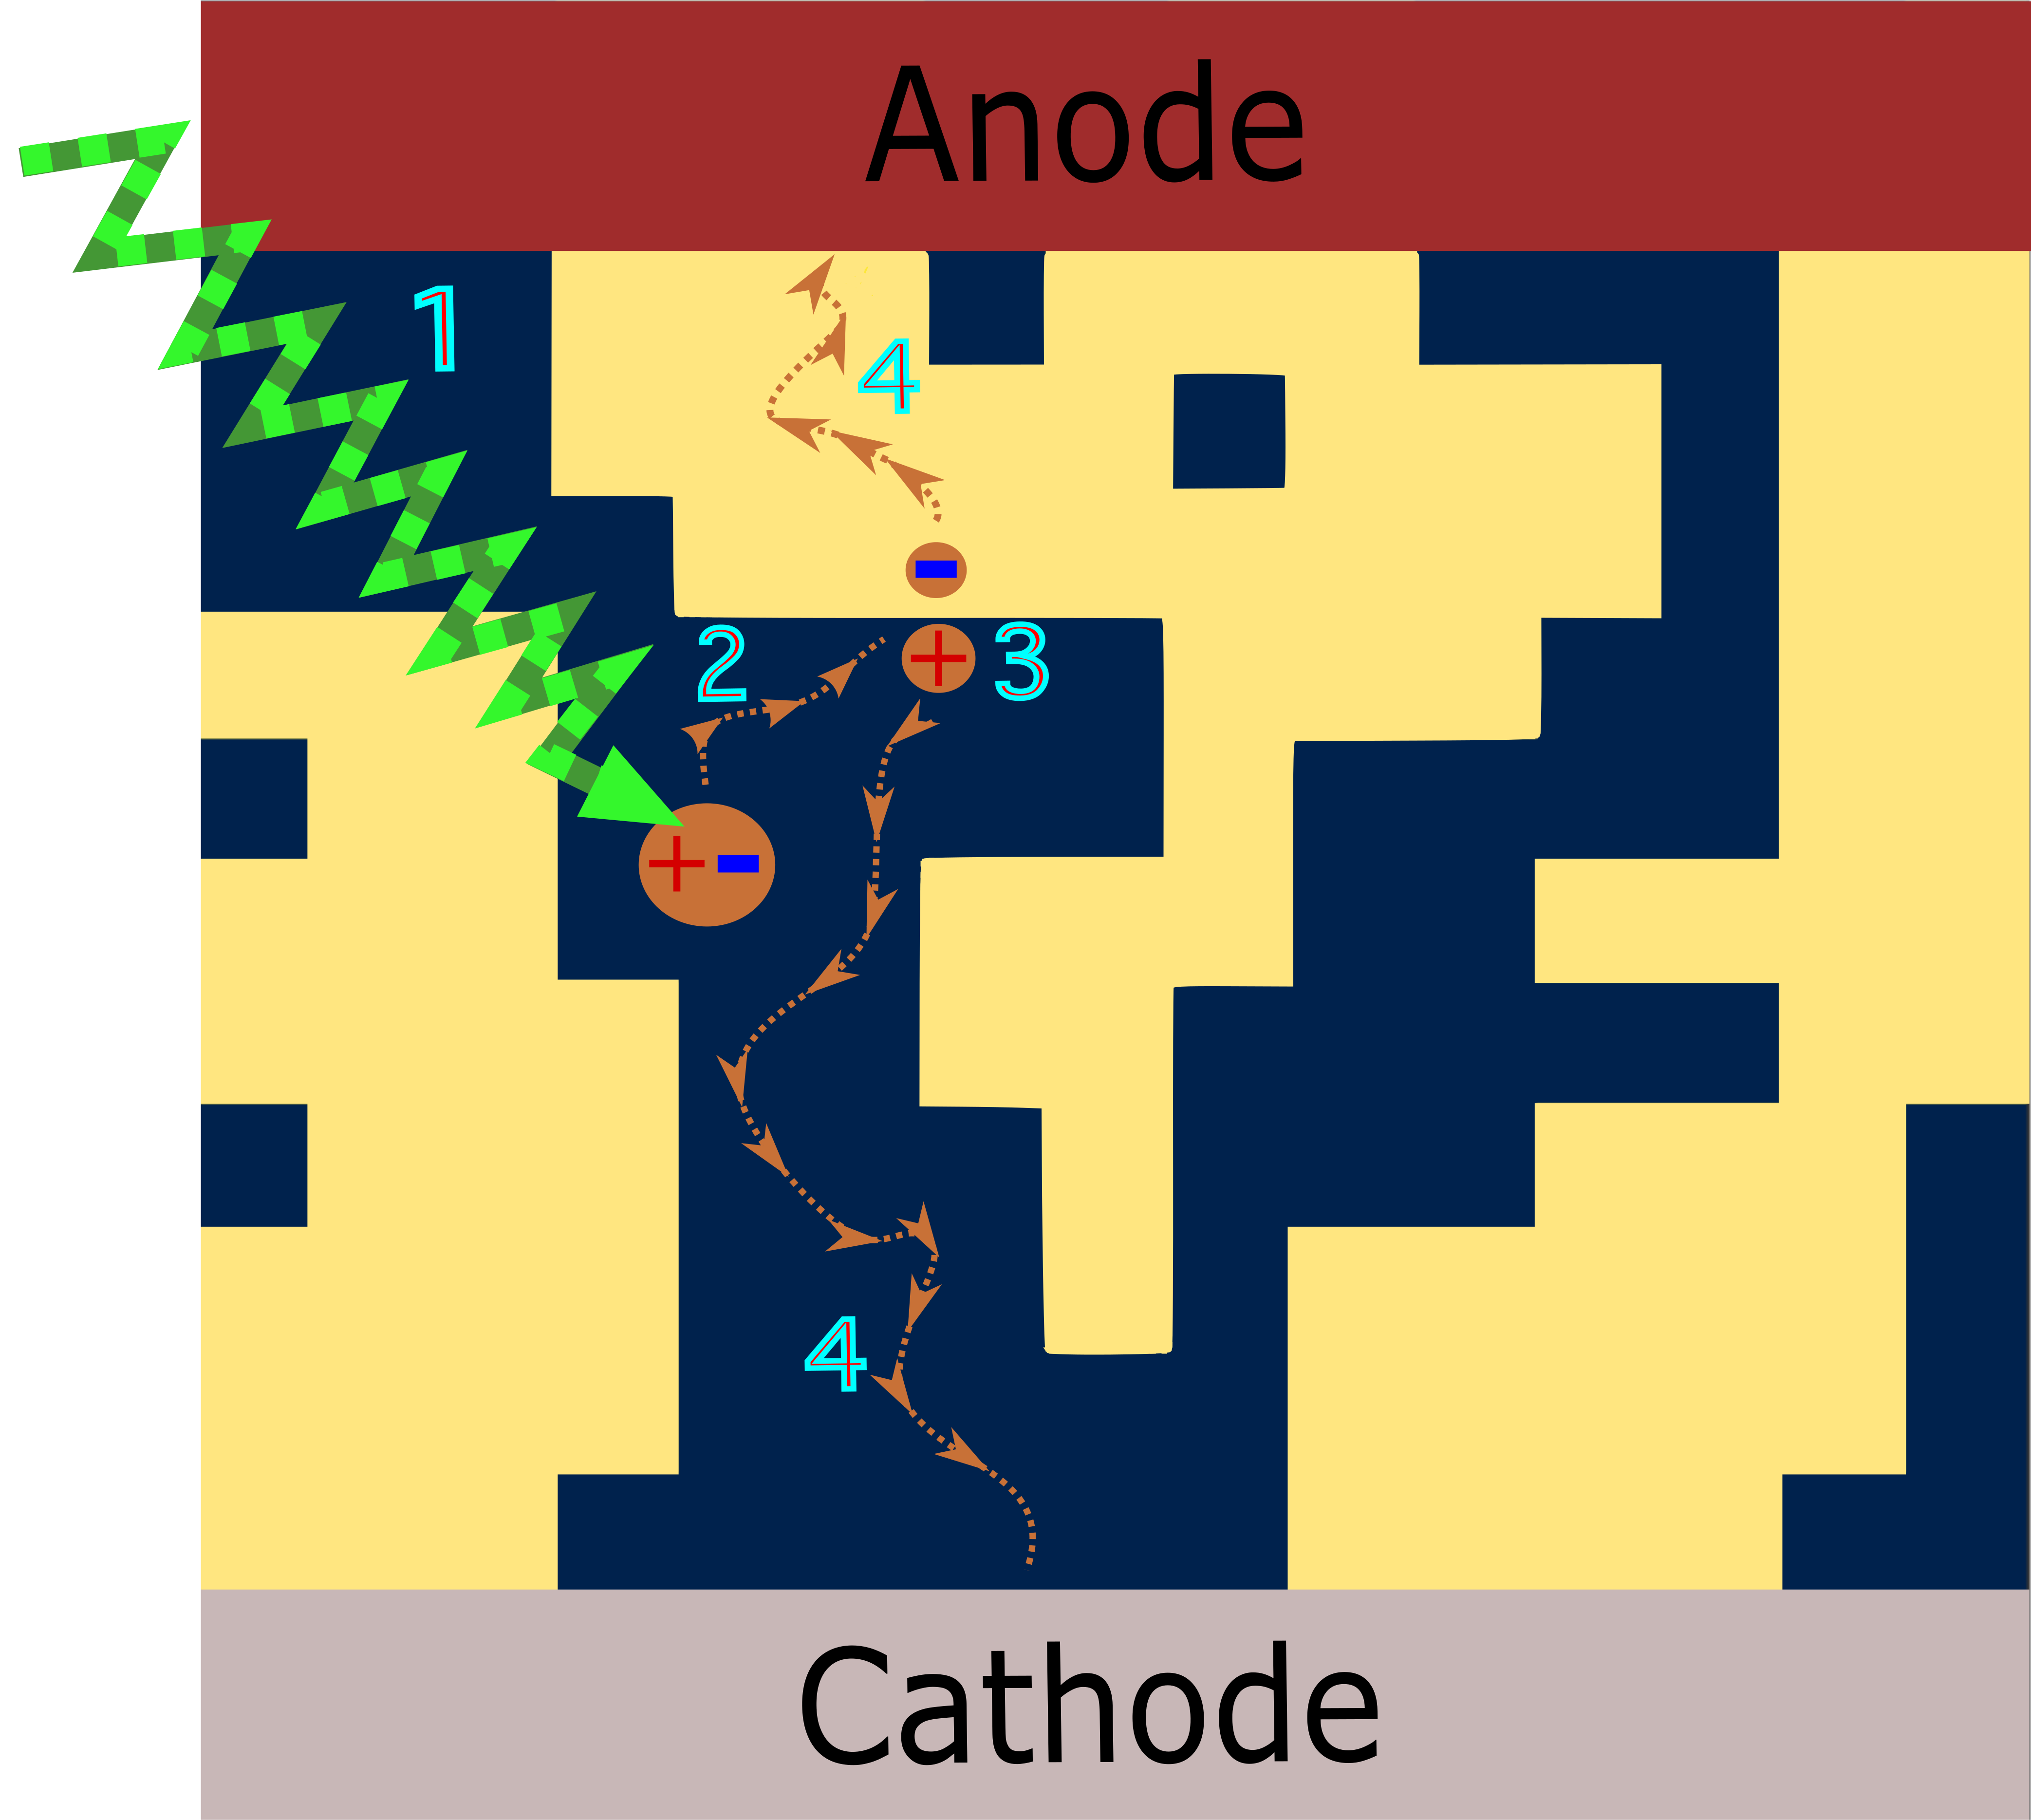
\includegraphics[width = .9\textwidth]{figures/BHJ-figure.png}
    \caption{A cartoon representation of a bulk heterojunction device. All four stages involved in harvesting
    photonic energy in a BHJ device are represtented. (1) The photon (green arrow) interacts with the material,
    exciting an electron and creating an quasiparticle referred to as an exciton. (2) The exciton diffuses
    about until it intersectects the interface between donor and acceptor material domains. (3) The exciton is
    coerced apart by the energy offset between donor and acceptor molecules. 
    (4) The, now unbound,  hole and the electron are free to diffuse about until ther reach their respective
    electrodes where they can be extracted \cite{Fusella2019}}
    \label{bhj}
\end{figure}

As shown in \ref{bhj}, a BHJ active layer proceeds through the following four stages: photoabsorbtions, 
exciton diffusion, charge transfer, and free charge diffusion \citet{Fusella2019}. When a photon is incedent on
an organic photovoltaic material, if it intersects with a molecular segment whose 
highest occupied molecular orbital (HOMO) has comprable energy levels to the photon, the energy can be absorbed via the promotion of
an electron to the next available energy level, the lowest unoccupied molecular orbital (LUMO).
This forms an exciton as
described above, which can then diffuse until it intersects the boundary. 
The excited electron would like to relax
back into is lower energy level, but at the interface with the acceptor, it finds a better option. The
acceptor's LUMO is engineered to sit between the energy of the donor's excited electron's energy level and the
available lower energy level. Because of this, the electron cascades down to the acceptors LUMO through a charge
tranfer reaction. Finally the free charges can diffuse until they interect the electrode where it can be
extracted. This is, of course, an ideal description. The are loss mechanisms at all four stages. 

Engineering the active layer of an OSC materials presents distinct challenges and advantages at
all four stages. Our work, however,  is most expressely related to stage four in that we seek to simulate free charges moving
through pure domains of donor or acceptor material. 

The BHJ design pushed the effenciency beyond the 1\% effeiciency milestone. Early BHJ devices utilized
fullerene derivitives as acceptors. In 2015, a group of researchers conceptulized the use of
fused-ring electron acceptors, a class of non-fullerene acceptors. This class of molecules consists of
a fused-ring core and end groups that can be engineered to acheive specific electronic characterstics and side
chains that can be engineered to achieve desried morphological features. The modularity of FREAs
layed the stage for headspinning progress in the following years from 4\% PCE to 18\%.
\cite{Wang2021a}

However reaching 18 \% effeciency in these devices required rigorous theory and 
time consuming chemical synthesis
that unfolded over the course of three decades. \ej{How'd theory play a role?} 
, it is desirable that a modular
open-source pipeline exhist for simulating the morphology of candidate molecules as well as simulating the 
associated charge charecteristics.\ej{Love it, but this is whiplash from the previous sentence. If we're pivoting to pipelines and screening now, then BHJ and NFA discussion is missing. I think maybe this sentence belongs elsewhere.} 
We note that will motivate zero-field mobility as a relvant quantity in BHJ
design, it could likely be informative accross all of the aforementioned applications. 


\ej{Like above, a bit of whiplash. Maybe get through all this intro first, and THEN explain where our work fits in.} Now, with the free electron bouncing around in the acceptor domain (the hole in the donor) how
quickly will it diffuse in that environement? This diffusivity, charge mobility, is what can be characterized in experiments and simulations and is one key metric for overall device efficiency.
%using MorphCT.

It has been show that the hole/electron mobility of both donor and acceptor material are
relavant to overall device performance. \cite{Wang2019e}. If electron mobililty is too high
in acceptor \ej{confusing} in comparison to the hole mobility in the donor, it gets clogged up and you get 
nongeminate recombination loss\ej{define?}.
Also, imbalanced charge-carrier mobility can lead to space-charge build up in the low mobilty material that
can screen the built in field.  \cite{Bartelt2015}. \ej{picture?}
This phenomena has been shown by space charge limited current eperiments \cite{Small2013}.

Taking for granted that electronic devices utilizing OPVs is an exciting
space, and with the immensity of the parameter space involved in molecular design, we find it highly desirable to have a pipeline through which we can simulate the equilibrium
chemistries of these materials and characterize their emergent material properties. Jones2017 has laid out this
pipeline in detail. To begin, equillibrium molecular dynamics (MD) simulations can predict the chemical
structure of OPVs. The data obtained from these simulations can then be fed as an input into kinetic monte
carlo (KMC) simulations that characterize charge mobility (conductivity) in these chemistries. We introduce MD
and our software stack used to implement it in \autoref{results}. The focus of this thesis, however, involves
the second leg of the pipeline; KMC simulation methods and software are explore in detail in autoref{results}.

Our KMC simulations are an implementation of the hopping model of electron transport.
The generic hopping model goes as follows: the wave functions of
free charges are localized on particular molecular segments, and the movements of these charges can be described as series
of hops bewtween these molecular segments. Where, and to what extent, charges delocalize can been investigated
[REFS]. In the \autoref{results} we explore the delineation of these segments, which we refer to as
``chromophore.'' 

The term chromophore arose in a biochemical context and is generally defined
as a light-absorbing group or molecule \cite{biochemistry}.
In this context, a chromophore is often associated with the color of a material.
This is because, mechanistically, a photon collides with a chromophore, the absorbed energy
excites an electron from the highest occupied molecular orbital (HOMO) to the
lowest unoccupied molecular orbital (LUMO). As the chromophore relaxes to its
ground state, it releases a photon with wave length $\lambda = \frac{\hbar c}{E}$,
where $\hbar$ is Plank's constant, $c$ is the speed of light, and $E$ represents the
energy difference of the HOMO and LUMO. 

For the materials of interest to our research, it would be undesirable for a chomophore to relax to its ground
state and release a photon, as this would consistute a loss mechanism. In the case of
OPVs we want our molecules bear that photo-electric
excitation long enough to jump to a nearby chromophore, and proceed, through a
series of quantum tunneling events, towards an electrode. 
In our work, a chromophore is defined as a region over which the
LUMO(HOMO for acceptor) of an excited molecular segment is thought to be fully delocalized. 
It is under this assumption that we execute a hopping model of charge transfer between
chromophores based on the Marcus rates of electrochemical reactions.  

\ej{Perhaps this is the place for a picture of the pipeline in terms of techniques/theory used, and we can get into our specifics later?}
\ej{This paragraph maybe belongs after the generic workflow description?}

Two open source python packages for
facilitating these two legs of the pipeline, Planckton and MorphCT, are maintained at 
the CMElab github repository \cite{cmelab}.
The use of Planckton in the methods and results sections below
constitute the experience of an end user as I had not personally developed this package before conscripting it
to do my MD simulating. Using Planckton-flow (also maintained on github), a sister package
of Planckton we took a container of planckton off the shelf and ran MD simulations of benchmark OPV
molecules on a high performance computing cluster without having to build the software stack or write the
simulation scripts from scratch. These packages are devloped with an emphasis on creating tools that are
transferable, reproducable, usable, and extensible (TRUE \cite{Cummings2017}).

My experience evinces what TRUE simulation engines can achieve and
informs the direction with which we seek to take MorphCT. We hope that the combination of these two packages
can make in silico experimentation with these materials realistically attainable by any aspiring researcher.
Having had no prior experience with these materials and/or materials simulation prior to joining the CMElab,
I was able to take an investigation of ITIC from molecular
structure to a charge mobility; a macroscopic property. 

Version one of MorphCT was capable of
connecting qualitativley the morphological features produced by MD simulations. However, it was determined
that in the interest of reprducabitilty, it was critical to ``containerize'' this pipeline. Until as recently as
the past few years it was common place to not publish code with the results of computational works. Containers
are virtual machines that contain all the dependencies, configurations, code and data necessary to reproduce
results. \cite{Cito2016a}

THIS SENTECE HAS NO HOME Researchers have to
balance the optimiztion of electron structures of candidate donor/acceptor materials against the miscibility
of two candidate molecules as well as the resultant morphology across the thermodynamic landscape of
variuos solution processes which ultimately govern the Jsc and FF of at the device level \cite{Zhu2020a}. 
\ej{After we show the generic pipeline of calculations that are needed, I think this is where we explain what specifically we do here: ``In this work we develop X for Y. In Section 2 we describe the theory and specific implementations of the methods used throughout the pipeline. In section 3 we report on experiments for validating and verifying our methods. In Section 4 we discuss the ramifications of this work and detail areas of future work.''}
%%% Local Variables: 
%%% mode: latex
%%% TeX-master: "BSUmain"
%%:set textwidth=80
% End: 
